%!TEX root = ../projektplan.tex
\chapter{Management Abläufe}

\section{Kostenvoranschlag}
\begin{itemize}
    \item Vier Entwickler während 14 Wochen
    \item Projektstart am 20. Februar 2014
    \item Projektende am 28. Mai 2014
    \item Aufwand Total: 14 Wochen * 10 Stunden * 8 Entwickler = 560 Stunden
\end{itemize}
Werden die Kernfunktionalitäten vorzeitig erfüllt, kann durch den Projektumfang die restliche Zeit vollumfänglich für optionale Funktionalitäten genutzt werden.

\section{Zeitliche Planung}
Wir werden in unserem Projekt nach dem Unified Process arbeiten. Die beinhaltet die Phasen: 
\\\begin{itemize}
    \item Inception
    \item Elaboration
    \item Construction
    \item Transition
\end{itemize}
\begin{figure}[ht]
    \center
    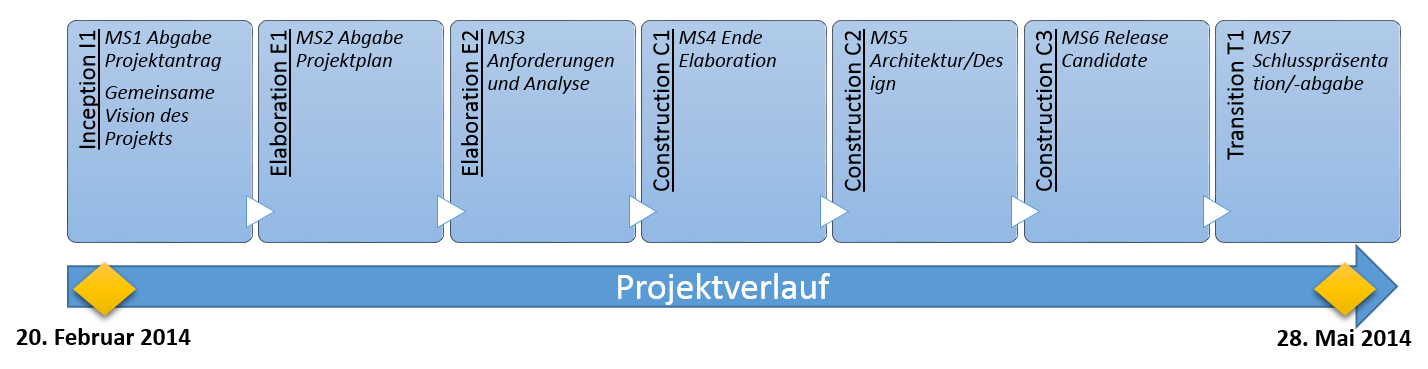
\includegraphics[width=\textwidth]{content/images/projektverlauf.png}
    \caption{Unified Process Phasen}
\end{figure}

\section{Iterationsplanung}
\begin{table}[H]
    \tablestyle
    \tablealtcolored
    \begin{tabularx}{\textwidth}{l X p{3.5cm} r}
        \tableheadcolor
            \tablehead Iteration &
            \tablehead Arbeitspaket &
            \tablehead Meilenstein &
            \tablehead SW \tabularnewline
        \tablebody
            \textit{Inception I1} &
            \begin{itemize}
                \item Projektantrag erstellen
                \item Virtueller Server beantragen
                \item Projektplan erstellen
                \item Entwicklungsumgebung einrichten (Client)
                \item Entwicklungsumgebung einrichten (Server)
                \item Vorgabe für Dokumentation erstellen
            \end{itemize} &
            \begin{itemize}
                \item MS1 Abgabe Projektantrag
                \item Gemeinsame Vision des Projekts
            \end{itemize} &
            1-2
        \tabularnewline
            \textit{Elaboration E1} &
            \begin{itemize}
                \item Projektplan verfeinern
                \item Domainanalyse
                    \begin{itemize}
                        \item Domainmodell
                        \item System State Diagramm
                        \item Operation Contracts
                    \end{itemize}
                \item Erstellen von Use Cases 
                    \begin{itemize}
                        \item Analyse
                        \item „brief“-Format zu 80%
                        \item „fully dressed“-Format zu 10%
                    \end{itemize}
                \item Erstellung Personas / Szenarios
                \item Anforderungsspezifikation erstellen
                \item Erstellung des Prototyps
                \item Machbarkeitsanalyse erstellen
            \end{itemize} &
            \begin{itemize}
                \item Abgabe MS2-RV. Projektplan
                \item MS3-RV. Anforderungen und Analyse
            \end{itemize} &
            2-4
        \tabularnewline
            \textit{Elaboration E2} &
            \begin{itemize}
                \item Entwicklungsumgebung vollständig eingerichtet
                \item Domainanalyse abgeschlossen
                \item Fertigstellung Anforderungsspezifikationen
                \item Fertigstellung Use Cases
                \item Fertigstellung Architektur-Prototyps
            \end{itemize} &
            &
            5-6
        \tabularnewline
            \textit{Elaboration E3} &
            \begin{itemize}
                \item Implementationsarbeiten beginnen
                    \begin{itemize}
                        \item Login-/Logout-Funktion
                        \item Für Helfereinsatz eintragen
                        \item Helfereinsätze planen
                    \end{itemize}
                \item Anpassungen gemäss Designreview
            \end{itemize} &
            \begin{itemize}
                \item MS4-RV. Ende Elaboration
            \end{itemize} &
            7-8
        \tabularnewline
        \tableend
    \end{tabularx}
    \caption{Iterationsplanung (1/2)}
\end{table}

\begin{table}[H]
    \tablestyle
    \tablealtcolored
    \begin{tabularx}{\textwidth}{l X p{3.5cm} r}
        \tableheadcolor
            \tablehead Iteration &
            \tablehead Arbeitspaket &
            \tablehead Meilenstein &
            \tablehead SW \tabularnewline
        \tablebody
            \textit{Construction C1} &
            \begin{itemize}
                \item Externes Design anpassen
                \item Implementationen erweitern
                    \begin{itemize}
                        \item Helfereinsätze importieren
                        \item Einsatzverwaltung
                    \end{itemize}
            \end{itemize} &
             &
            9-10
        \tabularnewline
            \textit{Construction C2} &
            \begin{itemize}
                \item Implementationen abschliessen
                    \begin{itemize}
                        \item Import- / Export-Funktionen
                        \item Optionale Funktionalitäten
                    \end{itemize}
                \item Testing 
                \item Reserven für Risiken
            \end{itemize} &
            \begin{itemize}
                \item MS5-RV. Architektur/Design
            \end{itemize} &
            11-12
        \tabularnewline
            \textit{Transition T1} &
            \begin{itemize}
                \item Präsentation vorbereiten
                \item Abschlussbericht verfassen
            \end{itemize} &
            \begin{itemize}
                \item MS6 Schlusspräsentation/-abgabe
            \end{itemize} &
            13-14
        \tabularnewline
        \tableend
    \end{tabularx}
    \caption{Iterationsplanung (2/2)}
\end{table}

\section{Meilensteine}

\subsection{MS1 Abgabe Projektantrag}
\begin{table}[H]
    \tablestyle
    \tablealtcolored
    \begin{tabularx}{\textwidth}{l X}
        \tablebody
        \tablehead Termin &
            21.02.14 (SW01) \tabularnewline
        \tablehead Phase &
            I1 \tabularnewline
        \tablehead Beschreibung  &
            Einreichung des Projektantrags und Genehmigung
            \tabularnewline
        \tablehead Deliverables  &
        	\begin{itemize}
                \item Projektantrag
            \end{itemize}
            \tabularnewline
        \tableend
    \end{tabularx}
    \caption{MS1 Abgabe Projektantrag}
\end{table}

\subsection{MS2 Abgabe Projektplan}
\begin{table}[H]
    \tablestyle
    \tablealtcolored
    \begin{tabularx}{\textwidth}{l X}
        \tablebody
        \tablehead Termin &
            06.03.14 (SW03) \tabularnewline
        \tablehead Phase &
            E1 \tabularnewline
        \tablehead Beschreibung  &
            Review Projektplan mit Zeitplan und aktuellen Iterationsplänen \tabularnewline
        \tablehead Deliverables  &
        	\begin{itemize}
                \item Projektplan mit Arbeitspaketen
            \end{itemize}
            \tabularnewline
        \tableend
    \end{tabularx}
    \caption{MS2 Abgabe Projektplan}
\end{table}

\subsection{MS3 Anforderungen und Analyse}
\begin{table}[H]
    \tablestyle
    \tablealtcolored
    \begin{tabularx}{\textwidth}{l X}
        \tablebody
        \tablehead Termin &
            13.03.14 (SW04) \tabularnewline
        \tablehead Phase &
            E1
            \tabularnewline
        \tablehead Beschreibung  &
            Review der Anforderungsspezifikation und Analyse \tabularnewline
        \tablehead Deliverables  &
        	\begin{itemize}
                \item Anforderungsanalyse
                \item Use-Case in Brief-Format
                \item Domainmodel
                \item Issues/Tasks in JIRA
            \end{itemize}
            \tabularnewline
        \tableend
    \end{tabularx}
    \caption{MS3 Anforderungen und Analyse}
\end{table}

\subsection{MS4 Ende Elaboration}
\begin{table}[H]
    \tablestyle
    \tablealtcolored
    \begin{tabularx}{\textwidth}{l X}
        \tablebody
        \tablehead Termin &
            10.04.14 (SW08) \tabularnewline
        \tablehead Phase &
            E2 \tabularnewline
        \tablehead Beschreibung  &
            Review der Dokumente und vorhandenen Code aus E1, E2 \& E3 \tabularnewline
        \tablehead Deliverables  &
        	\begin{itemize}
                \item Architektur-Prototyp
            \end{itemize}
            \tabularnewline
        \tableend
    \end{tabularx}
    \caption{MS4 Ende Elaboration}
\end{table}

\subsection{MS5 Architektur/Design}
\begin{table}[H]
    \tablestyle
    \tablealtcolored
    \begin{tabularx}{\textwidth}{l X}
        \tablebody
        \tablehead Termin &
            01.05.14 (SW11) \tabularnewline
        \tablehead Phase &
            C3 \tabularnewline
        \tablehead Beschreibung  &
           Review der Architektur/Design \tabularnewline
        \tablehead Deliverables  &
        	\begin{itemize}
                \item Dokument Architektur/Design
                \item Testplan
                \item Code RC Version
                \item Protokoll Code\-Reviews
            \end{itemize}
            \tabularnewline
        \tableend
    \end{tabularx}
    \caption{MS5 Architektur/Design}
\end{table}

\subsection{MS6 Schlusspräsentation/-abgabe}
\begin{table}[H]
    \tablestyle
    \tablealtcolored
    \begin{tabularx}{\textwidth}{l X}
        \tablebody
        \tablehead Termin &
            28.05.2013 (SW14) \tabularnewline
        \tablehead Phase &
            T1
            \tabularnewline
        \tablehead Beschreibung  &
            Durchführung der Schlusspräsentation \tabularnewline
        \tablehead Deliverables  &
        	\begin{itemize}
                \item Finales Produkt
                \item Präsentation
                \item Abgabe der Resultate
            \end{itemize}
            \tabularnewline
        \tableend
    \end{tabularx}
    \caption{MS6 Schlusspräsentation/-abgabe}
\end{table}

\section{Besprechungen}
Es wird wöchentlich mindestens eine fixe Teamsitzung mit allen Projektbeteiligten durchgeführt. Diese wird jeweils am Donnerstag stattfinden und zwischen ein bis zwei Stunden andauern. 
\\Sie dienen dem Zweck, getätigte Arbeiten mitzuteilen, bevorstehende Arbeiten gemeinsam zu planen und offene Fragen zu beantworten. Falls nötig, können weitere Sitzungen einberufen werden. 
\\Protokolle werden jeweils auf \href{http://www.minutes.io}{www.minutes.io} geführt und per E-mail an alle Projektmitarbeiter verteilt.
\\\begin{enumerate}
	\item Was haben wir erledigt?
	\item Welche nächsten Schritte stehen an?
	\item Wo gibt oder gab es Probleme, welche Entscheidungen wurden getroffen?
\end{enumerate}
Für Kurznachrichten im Team wird mit WhatsApp kommuniziert.
